\subsection{Low Level Design}

The low-level design explains the details of two modules; one is the interceptor module, and other is the sampling broker module. It further explains the interaction between the two modules.

\subsubsection{Interceptor Module}

Figure \ref{figures:artemis_interceptor} shows the class diagram for the interceptor module. The interceptor is named as Sampling Broker Interceptor. The Sampling Broker Interceptor is an incoming interceptor [\ref{subsubsection:in_interceptor}].

\makeatletter
\setlength{\intextsep}{20pt}
\makeatother

\begin{figure}[h!]
\centering
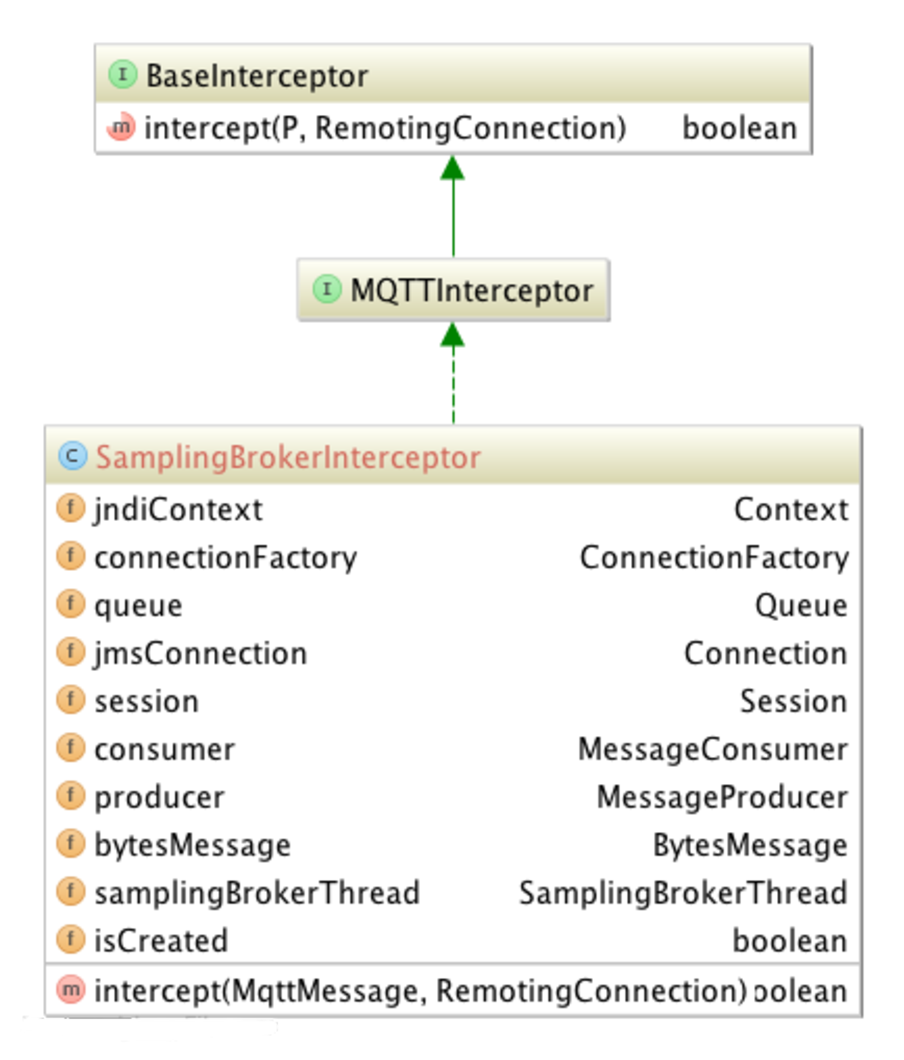
\includegraphics[keepaspectratio, width=0.6\textwidth, trim={0 0 0 0},clip]{interceptor.pdf}
\caption{Sampling Broker interceptor class diagram}\label{figures:artemis_interceptor}
\end{figure}

The Sampling Broker Interceptor implements the \textit{MQTTInterceptor} interface which enables it to receive all the incoming MQTT packets. The interceptor module sends the intercepted messages to a JMS queue using JMS.

\subsubsection{Sampling Broker Module}

\begin{figure}[h!]
\centering
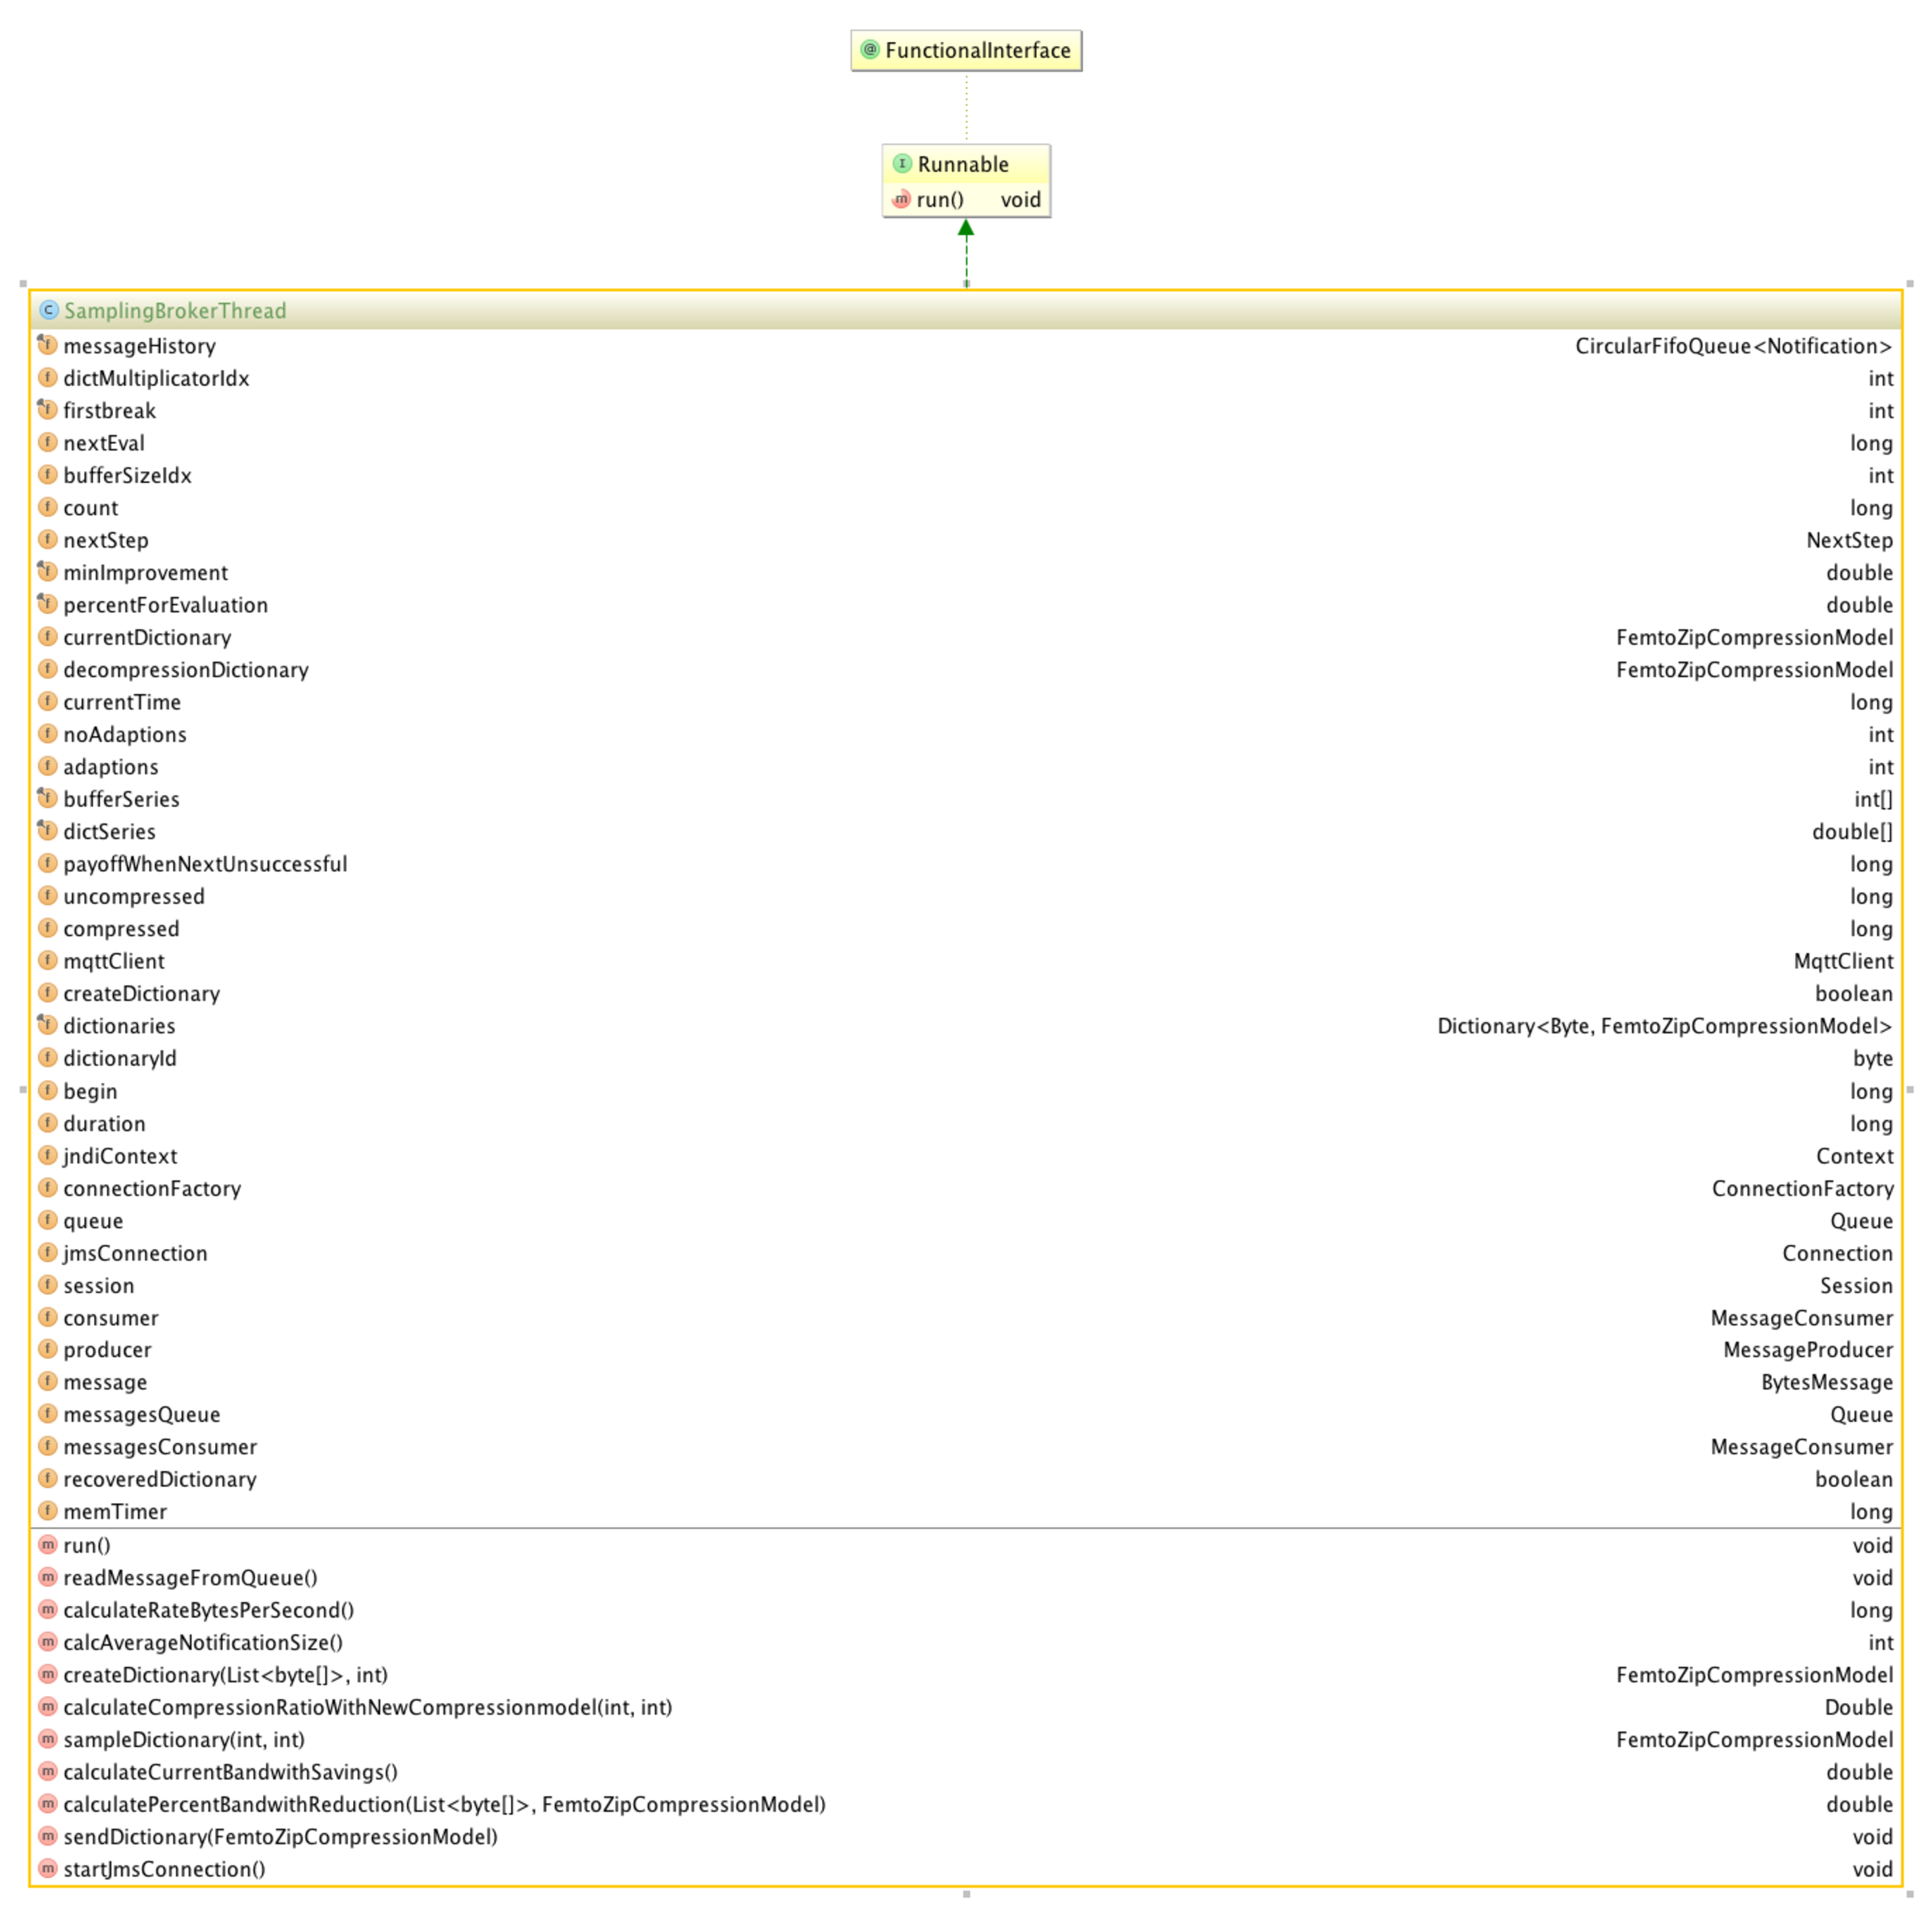
\includegraphics[keepaspectratio, width=1.0\textwidth, height=1.2\textheight, trim={0 0 0 0},clip]{thread.pdf}
\caption{Sampling Broker class diagram}\label{figures:artemis_thread}
\end{figure}

Figure \ref{figures:artemis_thread} shows the class diagram of the sampling broker module.

The sampling broker runs the adaptive sampling algorithm described in the section [\ref{subsection:algo}]. The sampling broker module gets the messages from a JMS queue via JMS.

\subsubsection{Interaction between modules} \label{subsubsection:interact}

The interaction between the interceptor module and the sampling broker module happens via JMS queues. The interceptor intercepts the messages and sends it to a JMS queue. The sampling broker then consumes the message from the same queue. 

\bigskip
\begin{lstlisting}[style=JavaInputStyle,caption=Interceptor sending message to JMS queue, label={lst:interact_code_send_queue}]
	public boolean intercept(MqttMessage packet, RemotingConnection connection) throws ActiveMQException {
		...
		bytesMessage = session.createBytesMessage();
		bytesMessage.writeBytes(msg);
		producer.send(bytesMessage);
		...
	    }
\end{lstlisting}

Listing \ref{lst:interact_code_send_queue} shows the code snippet used by the interceptor module to send the message to a JMS queue and Listing \ref{lst:interact_code_receive_queue} shows the code snippet used by the sampling broker to receive the message from the queue.

\bigskip
\begin{lstlisting}[style=JavaInputStyle,caption=Sampling Broker receiving message from \\ JMS queue, label={lst:interact_code_receive_queue}]
public void readMessageFromQueue() throws ActiveMQException {
        ...
        Message msg = messagesConsumer.receive(1);
        if (msg instanceof BytesMessage) {
            byte[] temp = new byte[(int) ((BytesMessage) msg).getBodyLength()];
            ((BytesMessage) msg).readBytes(temp);
            header = temp[0];
            payload = Arrays.copyOfRange(temp, 1, temp.length);
        }
        ...
    }
\end{lstlisting}

